Um motor de corrente contínua com velocidade constante pode ser representados pela figura \ref{fig:C1-21-II}.

\begin{figure}[ht!]
\center
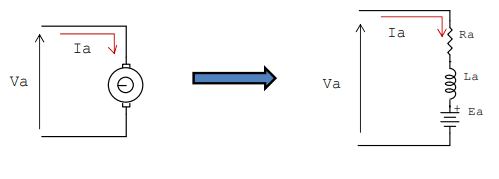
\includegraphics[scale= 0.88]{imagens/circuito1_21_II.png}
\caption{\label{fig:C1-21-II}Representação do motor CC com velocidade constante.}
\caption*{Fonte: MARTINS, cap. 5, eslaide 5.}
\end{figure}

Onde:

$R_{a} \rightarrow$ resistência de armadura.

$L_{a} \rightarrow$ indutância  de armadura.

$E_{a} = K_{a}\omega_{m} \rightarrow$ força contra-eletromotriz

Desta forma a figura \ref{fig:C2-21-II} representa um motor associado a um retificador controlado.

\begin{figure}[ht!]
\center
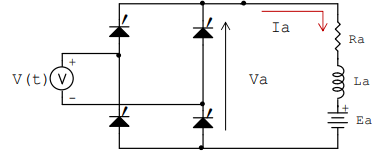
\includegraphics[scale= 0.88]{imagens/circuito2_21_II.png}
\caption{\label{fig:C2-21-II} Retificador controlado alimentando um motor CC operando com velocidade constante.}
\caption*{Fonte: MARTINS, cap. 5, eslaide 5.}
\end{figure}

Vale destacar que no acionamento dos motores CC considera-se os efeitos da condução descontínua.

\subsubsection{Ábaco de Pushlowski}
A figura \ref{fig:C1-22-II} representa a estrutura básica.

\begin{figure}[ht!]
\center
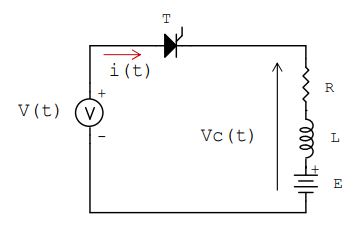
\includegraphics[scale= 0.88]{imagens/circuito1_22_II.png}
\caption{\label{fig:C1-22-II} Retificador monofásico controlado de meia-onda.}
\caption*{Fonte: MARTINS, cap. 6, eslaide 6.}
\end{figure}

E as formas de onda são (figura \ref{fig:G1-22-II}).

\begin{figure}[ht!]
\center
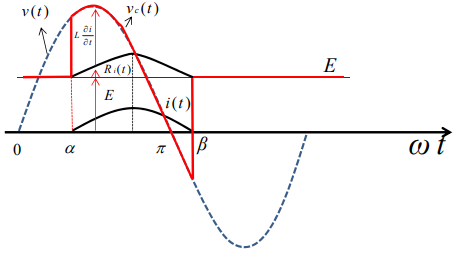
\includegraphics[scale= 0.88]{imagens/grafico1_22_II.png}
\caption{\label{fig:G1-22-II} Principais formas de onda.}
\caption*{Fonte: MARTINS, cap. 5, eslaide 6.}
\end{figure}

Onde:

$\alpha \rightarrow$ ângulo de disparo do tiristor.

$\beta \rightarrow$ ângulo de extinção do tiristor.

$\gamma = \beta - \alpha \rightarrow$ ângulo de condução.

\[v(t) = \sqrt{2}V\sin{\omega_{t}}\]

Onde V é o valor eficaz da tensão de entrada v(t).

Quando o tiristor conduz, no intervalo $(\alpha,\beta)$, a corrente é determinada pela seguinte equação:
\[v(t) = Ri(t) + L\frac{di(t)}{dt} + E\]

A solução dessa equação é dada por:

\[i(t) = \frac{\sqrt{2}V}{R}\left[\cos{\theta}\sin({\omega{t} - \theta}) - a + \left[a - \cos{\theta}\sin({\alpha - \theta})\right]e ^{-\frac{(\omega{t} - \alpha)}{\tan{\theta}}}\right]\]

\[a = \frac{E}{\sqrt{2}V}\]
\[\theta = \tan^{-1}{\frac{\omega{L}}{R}}\]

É importante salienta que o parâmetro "$a$" é proporcional a velocidade do motor CC $\rightarrow$ coeficiente de velocidade do sistema Retificador-Motor.

E, para $\omega{t} = \beta \Rightarrow i(t) = 0$. Portanto:

\[\left[\cos{\theta}\sin({\beta - \theta}) - a + \left[a - \cos{\theta}\sin({\alpha - \theta})\right]e ^{-\frac{(\beta - \alpha)}{\tan{\theta}}}\right] = 0\]

Nenhuma das variáveis da equação anterior podem ser explicitadas, portanto, utiliza-se o ábaco de Puschlowski (figura \ref{fig:A-22-II} que representa essa mesma equação para todos os retificadores a tiristor. Essa mesma expressão também pode ser solucionada numericamente.


\begin{figure}[ht!]
\center
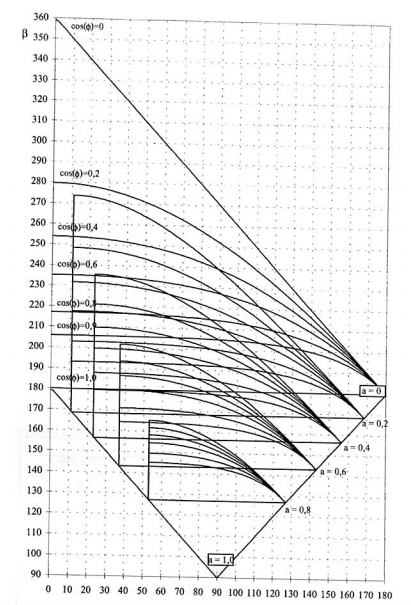
\includegraphics[scale= 0.88]{imagens/abaco_22_II.png}
\caption{\label{fig:A-22-II} Ábaco de Puschlowski.}
\caption*{Fonte: MARTINS, cap. 5, eslaide 8.}
\end{figure}


A condução torna-se crítica quando:

\[ \gamma_{c} = \frac{2\pi}{p}\]

Onde:

$\gamma_{c} \rightarrow$ ângulo de condução crítica.

$p \rightarrow$ número de pulsos do retificador.

Como: $\gamma_{c} = \beta_{c} - \alpha_{c} \Rightarrow \alpha_{c} = \beta_{c} - \frac{2\pi}{p}$

No ábaco da figura \ref{fig:A-22-II} obtém-se o valor de $\cos{\theta}$ e $\theta$. E, com a relação $\tan{\theta} = \frac{\omega{L}}{R}$, determina-se o valor da indutância crítica $L_{c}$.

Com $L_{c} = L_{ext} + L$, é possível determinar a indutância externa para manter a condução contínua.

\subsubsection{Estruturas dos retificadores em questão}

\begin{figure}[ht!]
\center
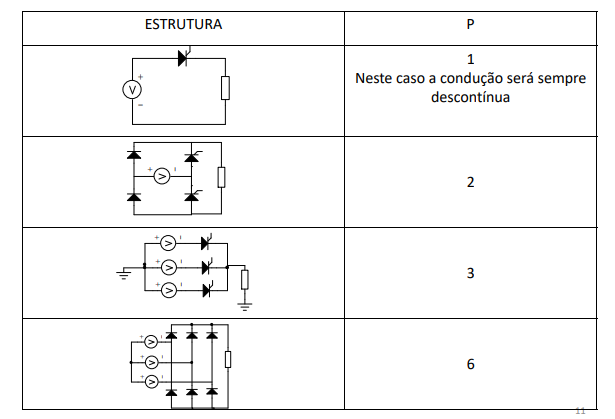
\includegraphics[scale= 0.88]{imagens/tabela1_24_II.png}
\caption{\label{fig:T-24-II} Estruturas retificadoras.}
\caption*{Fonte: MARTINS, cap. 5, eslaide 11.}
\end{figure}

\subsubsection{Cálculo das tensões médias}

A tensão média produzida pelo retificador é dada pela seguinte expressão:
\[E_{dc} = \frac{1}{2\pi}{p} \int_{\alpha}^{\beta}\left(\sqrt{2}V\sin{\omega{t}}\right)d\omega{t}\]

Ou seja,
\[E_{dc} = \frac{\sqrt{2}}{2}\frac{p.V}{\pi}\left(\cos{\alpha} \cos{\beta}\right)\]

Quando a condução é contínua obtém-se:

\[\beta = \alpha + \frac{2\pi}{p}\]

Logo:

\[E_{dc} = \frac{p.V}{\sqrt{2}\pi}\left[\cos{\alpha} - \cos{\left(\alpha + \frac{2\pi}{p}\right)}\right]\]

A tensão média nos terminais da máquina é dada por:

\[E_{dc}' = RI_{dc} + E \]
\[RI_{dc} = E_{dc}' - E = \frac{p}{2\pi}\int_{\alpha}^{\beta}\left(\sqrt{2}V\sin{\omega{t} - E}\right)d\omega{t} \]

Portanto:

\[E_{dc}' = \frac{pV}{\sqrt{2}\pi}\left[\cos{\alpha} - \cos{\beta} - \frac{E}{\sqrt{2}V}\frac{2\pi}{p}\right]\]

Quando a condução é contínua $E_{dc}' = E_{dc}$.

\subsubsection{Expressão clássica da tensão}
Representa-se um ângulo de disparo $\psi$ definido de acordo com o número de pulsos do retificador. Assim, conforme a figura \ref{fig:G1-252-II}, tem-se:
\[Z = \frac{p\pi - 2\pi}{2p}\]

\begin{figure}[ht!]
\center
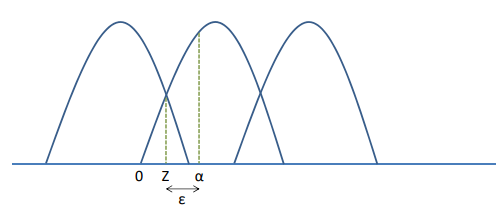
\includegraphics[scale= 0.88]{imagens/grafico1_252_II.png}
\caption{\label{fig:G1-252-II} Forma de onda da tensão oriunda de um retificador trifásico}
\caption*{Fonte: MARTINS, cap. 5, eslaide 15.}
\end{figure}

Deste modo,

\[Z + \psi = \alpha \Rightarrow \psi = \alpha - \frac{p\pi - 2\pi}{2\pi}\]

Portanto:

\[E_{dc} = \frac{p.V}{\pi.\sqrt{2}}\left[\cos\left(\psi + \frac{\pi.p - 2\pi}{2p}\right) - \cos\left(\psi + \frac{\pi}{2} - \frac{\pi}{p} + \frac{2\pi}{p}\right)\right]\]

\[E_{dc} = \frac{\sqrt{2}.p.V}{\pi}\left[\sin\left(\frac{\pi}{p}\right)\cos{(\psi)}\right]\]

Essa última é a expressão clássica para os retificadores , válida somente para condução contínua e p>1.

Para $\frac{\pi}{2} < \psi < \pi  \Rightarrow E_{dc} < 0$

Isso significa que o conversor funciona como inversor não autônomo; e a máquina pode fornecer energia á rede nessa condição. 

\subsubsection{Excitação separada e retificador a tiristor (caso geral)}

Parte-se da estrutura conforme na figura \ref{fig:C1-26-II}.

\begin{figure}[ht!]
\center
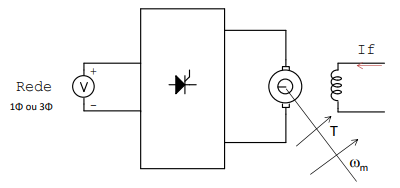
\includegraphics[scale= 0.88]{imagens/grafico1_26_II.png}
\caption{\label{fig:C1-26-II} Motor CC alimentado por retificador a tiristor}
\caption*{Fonte: MARTINS, cap. 5, eslaide 16.}
\end{figure}

Conhecendo-se os parâmetros do motor, deseja-se determinar a sua característica torque-velocidade quando associado ao retificador. Portanto foi estabelecido que para a condução descontínua:

\[\frac{RI_{dc}}{\sqrt{2}V} = \frac{p}{2\pi}\left[\cos\alpha - \cos\beta - a(\beta - \alpha)\right]\]

E, para condução contínua,

\[\frac{RI_{dc}}{\sqrt{2}V} = \frac{p}{2\pi}\left[\cos\alpha - \cos\left(\alpha + \frac{2\pi}{p}\right) - a\frac{2\pi}{p}\right]\]

Para um $I_{f}$ constante $\Rightarrow T = f(I_{dc})$. Ou seja, o torque é proporcional a $I_{dc}$. Portanto:
\[\frac{R}I_{dc}{V\sqrt{2}} = t_{f}\]

$t_{f}$ é o fator de torque.

Desse modo obtém-se:

$t_{f} = \frac{p}{2\pi}\left[\cos{\alpha} - \cos{\beta} \alpha\left(\beta - \alpha\right)\right] \rightarrow$ para condução contínua.

$t_{f} = \frac{p}{2\pi}\left[\cos{\alpha} - \cos\left(\alpha + \frac{2\pi}{p}\right) - a.\frac{2\pi}{p} \right] \rightarrow$ para condução descontínua.

Sendo assim, pode-se obter um conjunto de características $t_{f} = f(a)$, onde p é fixado e $\alpha$ é considerado um parâmetro. 

Para condução contínua, utiliza-se a primeira definição de $t_{f}$. E, quando a condução é descontínua, para um dado $\alpha$ deve-se calcula $\beta$ a partir do ábaco de Pushlowski, para em seguida determinar $t_{f}$

